% !TEX root = catron-dissertation.tex
\epstopdfsetup{outdir=./images/04_dispersion_analysis/}

\chapter{Multidimensional Spectral Estimation of Optical Wavefronts}
\label{chap:04_dispersion}
% \begin{itemize}
%   \color{red}
%   \item
% \end{itemize}

As described in Chapter \ref{chap:01_intro}, the objective of this research is to develop methods to evaluate and, if possible, eliminate the effect of facility-related acoustic noise on aero-optical measurements.
As such, the first goal of the research is to establish analytical methods to identify and isolate acoustic sources of optical signals within a given data sample.
This is a significant challenge since, as will be shown later, acoustic sources of optical aberrations typically have a magnitude and frequency content that is in the same range as the signal that is the objective of the measurement.
This chapter will begin with a brief overview of some of the benefits to analyzing multidimensional data in this way, followed be a short discussion on how these spectrum are calculated, and conclude with a more in depth discussion on the analysis of multidimensional spectral estimates.


The multi-dimensional spectral approach that is employed throughout this research helps identify and characterize acoustic sources of optical noise as well as aero-optical signals.
The spectral approach is also used as the basis for methods to filter the acoustic sources.
For measurements in multiple dimensions, such as a line of sensors that are recorded over time, a multidimensional spectral estimation not only produces temporal frequency content but can also be used to identify the direction and speed of travel of a particular wave.
The benefits of using multidimensional spectral estimation are shown in Figure \ref{fig:04_dispersion_demo}.
\begin{figure}
\centering
  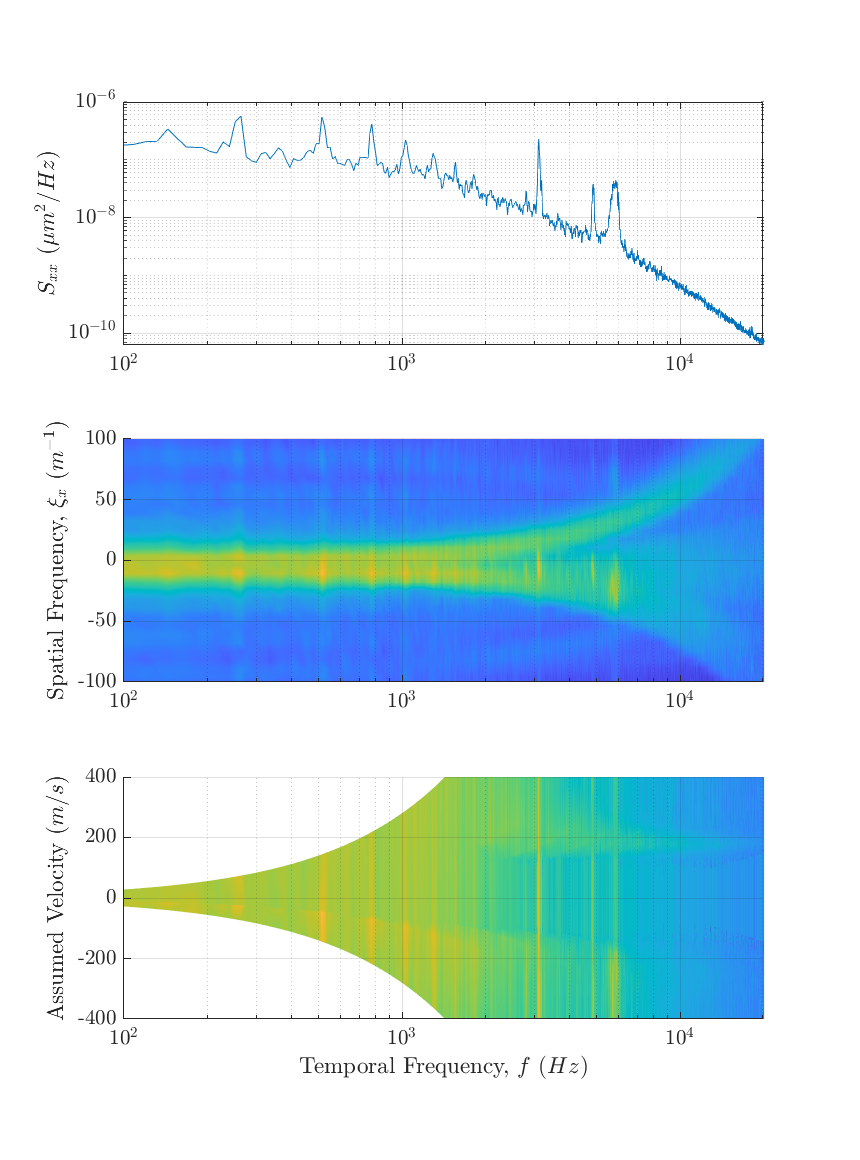
\includegraphics{../matlab/04_dispersion_analysis/dispersion_demo.eps}
  \caption{Multidimensional spectral estimation plot example and comparison to traditional power spectrum measurements. A single row of an optical wavefront measurement was used in this example. The top plot shows the typical power spectrum averaged over the entire row of data. Both the middle and bottom plots show the multidimensional spectrum plot with the y-axis as spacial-frequency in the middle and velocity in the bottom assuming $u=f/\xi_x$.}
  \label{fig:04_dispersion_demo}
\end{figure}
A single row of sub-apertures was from an optical wavefront measurement with a 5 inch diameter beam propagating normally through a wind-tunnel test section with a free-stream Mach number of 0.5.
This measurement was preformed in the University of Notre Dame Whitefield Wind Tunnel in a test section that contained a model representing the fuselage of the AAOL aircraft \cite{Jumper-2013-8KtN3pue} with window that was flat and flush to the outer mold line of the fuselage.
The top plot shows a traditional power spectrum ensemble-averaged over the row of data.
Both the blade-passing frequency (517 Hz) and its sub-harmonic had similar amplitudes  with an additional five harmonics showing significant spikes above the local baseline measurement.
There are three additional strong peaks at approximately 3100, 4850, and 5850 Hz that are likely due to additional fan vibration that is currently limiting the top speed of the tunnel.

Both the middle and bottom plots show the multidimensional spectral estimation plot of  two-dimensional measurement.
The colorbars were intentionally not shown in order to allow for all three plots to be aligned in the temporal-frequency axis and the color is representative of the logarithm of the power or variance in the wavefront signal (i.e. $\opdrms^2$) with yellow representing more power and blue representing less.
The colorbar range in this plot is the same is constant with the other plots throughout this chapter.
In the middle plot the y-axis represents the stream wise spatial frequency, $\xi_x$ with the units of inverse meters.
It is important to note that, unlike temporal-frequencies, spatial-frequencies can have positive or negative values depending on the direction of travel of the disturbance; this means that, waves with positive spatial-frequencies are moving in the direction of flow.
The upstream and downstream traveling signals begin to diverge at around 2000 Hz with the signal below that point primarily laying on the upstream traveling side of the plot.
The blade-passing frequency and its various harmonics can also be discerned in the center plot, by the vertical ``streaks'' that line up  with the peaks in the standard spectrum shown in the top plot; the center spectral plot shows that these fan blade-passing signals have significant broadband spatial-frequency content.
All of these narrow-band signals have a majority of their signal traveling upstream.
In addition to optical disturbances branching off in the upstream and downstream moving directions there are significant disturbances along zero spatial-frequency representing a collection of standing waves.
Elsewhere in this paper the multidimensional spectral estimation will be plotted with the temporal-frequency axis linearly.
This data has been plotted logarithmically along the temporal-frequency axis to better slow the low frequency content.
When plotted linearly, the two primary upstream and downstream traveling signals lay in a straight line.

A dispersion analysis can be performed on these multidimensional spectral estimates.
In order to obtain the velocity of a given wave we can start with the most basic forms of the wave equation,
\begin{equation}
  \hat{y} = a\exp\{j\theta\} \textrm{,}
\end{equation}
where $\theta$ is the phase of the wave and equal to $kx-\omega t$.
From here we can take the partial of $\theta$ with respect to time and set it equal to zero,
\begin{equation}
  \frac{\partial\theta}{\partial t} = 0 = \frac{\partial k}{\partial t}\frac{\partial x}{\partial t}-\frac{\partial \omega}{\partial t}\frac{\partial t}{\partial t} \textrm{,}
\end{equation}
which can be rearranged to
\begin{equation}
  u = \frac{\partial \omega}{\partial k} = \frac{\partial f}{\partial \xi} \textrm{.}
\end{equation}
If we are to assume that a wave packet intercepts the origin ($f=\xi=0$) then every point on the spectral plot can be labeled with an assumed velocity,
\begin{equation}
  u_{assumed} = \frac{f}{\xi_x} \textrm{.}
  \label{eqn:04_velocity_assumed}
\end{equation}

The bottom plot shows the same multidimensional spectral estimation plot as the middle one but with the y-axis representing an assumed velocity.
There is not much in the way of velocity measurement capability at low temporal-frequencies
The primary optical disturbance moving in the direction of flow is moving at the free-stream velocity of approximately 175 m/s.
The upstream traveling disturbance is traveling at the same speed but due to the signal being broader is more difficult to measure this way.
The stationary modes in the middle plot are nowhere to be found on the bottom plot.
When the assumed velocity for this these waves is calculated their speed approaches infinity.

%bookmark
\section{One-Dimensional Power Spectrum Calculation}
Power spectral analysis is typically performed on one-dimensional data sets, for example, a single sensor measurement over time.
On the other hand, if a sensor array were used, a multi-dimensional power spectrum could be computed that would also show spatial frequency information at each instant in time.
For a single-point measurement that varies in time, $x(t)$, the power spectrum calculation is
\begin{equation}
 S_{xx} = \frac{|\fft\{x(t)\}|^2}{Nf_{s}} \textrm{,}
 \label{eqn:04_basic_sxx}
\end{equation}
where $\fft$ is the Fast Fourier Transform, $N$ is the number of samples, and $f_{s}$ is the sample rate \cite{Blackman-1958-4QtKgDb8}.
For data that has only a real component the Fast Fourier Transform function produces magnitude and phase relations at each frequency step, $f_{s}/N$, over the range from zero-frequency up to but not including the Nyquist frequency, $f_s/w$, with a mirrored set of data that can be represented either below (starting at $-f_s/2$) or above (ending just below $f_s$) this range.
The Nyquist frequency not being included and the mirrored data is due to an assumption that is integral to the Fourier Transform, which is that the signal is assumed to be periodic.

The total energy, $\sigma^2$, of the signal must be preserved through the transform from physical space-time to frequency space
\begin{equation}
  \sigma^2 = \frac{\sum x^2(t)}{N} = \Delta f\sum S_{xx}(f) \textrm{.}
  \label{eqn:04_fft_energy_conservation}
\end{equation}
Additionally, because of the periodic nature of the Fourier Transform and a finite sample length of discrete data, spectral leakage can cause the power in one frequency bin to leak into adjacent frequency bins.
To minimize this spectral leakage, windowing functions are employed which typically force the end points of the signal to zero.
The Hann window,
\begin{equation}
 w(t) = 1/2\left[1-\cos\left(\frac{2\pi t}{T}\right)\right] \textrm{,}
 \label{eqn:04_hann_window}
\end{equation}
is one of the more commonly used windowing functions \cite{Braun-2001-qhqBfvYz} where $w(t)$ is the window function, $t$ is the time at a given sample, and $T$ is the total sample time.
Since the windowing of a data set changes the signal energy some correction is needed to be applied.
For an arbitrary windowing function the correction factor, $c_w$, can be obtained by substituting the windowing function in place of $x(t)$ in Equation \ref{eqn:04_fft_energy_conservation},
\begin{equation}
 c_w = \frac{1}{\sqrt{\sum w^2(t)/N}} \textrm{.}
 \label{eqn:04_window_correction}
\end{equation}
For a Hann window this correction factor approaches $\sqrt{8/3}$ as $N$ goes to infinity.
When Equation \ref{eqn:04_basic_sxx} is combined with a windowing function and associated correction the double sided power spectra equation in one dimension becomes
\begin{equation}
 S_{xx} = \frac{|c_w\fft\{x(t) w(t)\}|^2}{Nf_{s}} \textrm{.}
 \label{eqn:04_windowed_sxx}
\end{equation}
A simple MATLAB function for computing the power spectrum of a one-dimensional signal with an arbitrary windowing function is shown in Appendix \ref{code:sc_simpleSXX}.

\section{N-Dimensional Power Spectra Calculation}
For measurements with multiple spatial and temporal dimensions the Fast Fourier Transform is applied $n$-times where $n$ is the total number of dimensions, with each application in a different dimension,
\begin{equation}
 \fftn(x) = \fft(\fft(\cdots\fft(\fft(x,1),2)\cdots,n-1),n) \textrm{,}
 \label{eqn:04_fftn}
\end{equation}
where $\fft(x,n)$ is the Fast Fourier Transform of $x$ in the $n^{th}$ dimension \cite{An-1991-QKg7heKm}.
For a $n$-dimensional array the operation becomes \cite{McClellan-1982-rGQzuZ7t}
\begin{equation}
 \mathbf{S_{xx}} =\frac{|c_w\fftn\{f(\mathbf{x}) w(\mathbf{x})\}|^2}{\prod{\overrightarrow{N}\overrightarrow{f_s}}} \textrm{,}
 \label{eqn:04_sxxn}
\end{equation}
where $\mathbf{S_{xx}}$ is the $n$-dimensional power spectra array or dispersion array, $f(\mathbf{x})$ is a $n$-dimensional set of data, $w(\mathbf{x})$ is a $n$-dimensional windowing function, $\overrightarrow{N}$ is a vector denoting the number of elements in each dimension, $\overrightarrow{f_s}$ is a vector denoting the sample rate in each dimension, and
\begin{equation}
 c_w = \frac{1}{\sqrt{\sum w^2(\mathbf{x})/\prod{\overrightarrow{N}}}} \textrm{.}
 \label{eqn:04_windown}
\end{equation}
The signal energy conservation relationship becomes
\begin{equation}
  \sigma^2=\frac{\sum\mathbf{x}}{\prod{\overrightarrow{N}}} = \prod{\overrightarrow{\Delta f_s}}\sum\mathbf{S_{xx}} \textrm{,}
  \label{eqn:04_fftn_energy_conservation}
\end{equation}
where $\overrightarrow{\Delta f_s}$ is a vector representing the frequency step sizes in each dimension.
A simple MATLAB code for calculating the dispersion of $x$ with an arbitrary windowing function is shown in Appendix \ref{code:sc_simpleSXXn}.

\section{Non-Rectangular Spatial Windows}
For n-dimensional data sets that fill a rectangular array, a windowing function can be created by multiplying together a series of one-dimensional windowing functions in the direction of each dimension.
For non-rectangular data sets, such as is often the case with optical wavefront measurements, a windowing function can take some additional steps in its construction.
In cases when the spatial measurement locations are constant throughout time, the windowing function can be split into two separate components,
\begin{equation}
 w(\mathbf{x}) = w_t(t)\cdot w_s(x,y) \textrm{,}
 \label{eqn:04_window_sep}
\end{equation}
the temporal windowing function, $w_t(t)$, and the spatial windowing function, $w_s(x,y)$.
This study uses a Hann window for the temporal windowing function and a modified Hann window for the spatial windowing function.
For the case of a perfectly circular aperture, the Hann window can be reformulated to be based on the normalized radius, $\rho_N$, of the aperture,
\begin{equation}
 w_s(\rho_N) =
 \begin{cases}
  \frac{1+\cos(\pi\cdot\rho_N)}{2} & \textrm{if } \rho_N < 1 \\
  0                                & \textrm{otherwise.}
 \end{cases}
 \label{eqn:04_window_space}
\end{equation}
This modified Hann window is two-dimensional with a value of one at the center of the aperture and decreases to zero at the edge of the aperture in the same manner as a Hann windows decreases from the center to either end.

Because the wavefronts measurements often had a clipped edge or some other obscuration, a different method was employed in this study.
For an arbitrary shaped aperture, the minimum distance from any given measurement location to the edge of the aperture was used to create the spatial windows.
The minimum distance can be computed given the a set of points ($x$ and $y$) that spans the measurement range and the set of points outside of the aperture ($x_O$ and $y_O$),
\begin{equation}
 d_{min}(x,y) = \min\left\{\sqrt{(x-x_{O})^2+(y-y_{O})^2}\right\} \textrm{.}
 \label{eqn:04_window_space_arb_dist}
\end{equation}
This distance is then normalized by the maximum value and the resulting spatial window given a modified Hann window,
\begin{equation}
 w_s(x,y) = \frac{1+\cos\left\{\pi\cdot\left(1-d_{min}^{norm}(x,y)\right)\right\}}{2} \textrm{.}
 \label{eqn:04_window_space_arb}
\end{equation}
% An arbitrary aperture and its corresponding spatial window are shown in Figure \ref{fig:04_spatial_window}.
% \begin{figure}
%   \centering
%   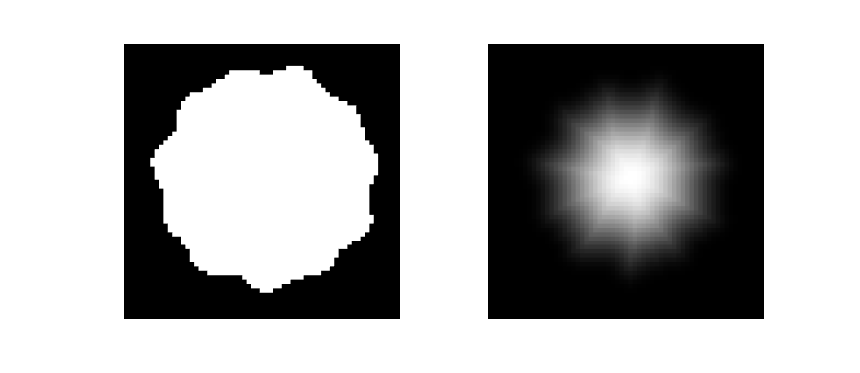
\includegraphics{../matlab/04_dispersion_analysis/spatial_window.eps}
%   \caption{An arbitrary nearly round aperture and its corresponding spatial window.}
%   \label{fig:04_spatial_window}
% \end{figure}
% This aperture is nearly circular with slight perturbations along the edge.
This same basic idea can be extended to data sets where the locations of measurements in space vary with time.

\section{Wavefront Multidimensional Spectrum}
At the beginning of this chapter a multidimensional spectral plot for data resolved in time and one spatial dimension was shown along with a typical power spectrum plot in Figure \ref{fig:04_dispersion_demo}.
This was shown to facilitate a simple discussion of some of the benefits of using multidimensional spectrum analysis on optical wavefronts.
That simple analysis was performed on only a single row of a wavefront data set and provided an insight into the disturbances that were moving in the horizontal (stream wise) direction only.
When multidimensional spectral estimation is performed over all dimensions of a wavefront (i.e. time and both spatial dimensions), as will be done for the remainder of this chapter, additional detail is available, that also enables the determination of optical disturbances moving vertically (i.e. cross-stream to the flow) or any direction in between.
Figure \ref{fig:04_dispersion_comparison} shows a comparison between the two-dimensional single row spectrum and a three-dimensional spectral slice showing the horizontal moving optical disturbances at both zero-vertical spatial frequency and integrated through the vertical spatial frequencies in order to obtain the two-dimensional spectrum.
\begin{figure}
  \centering
  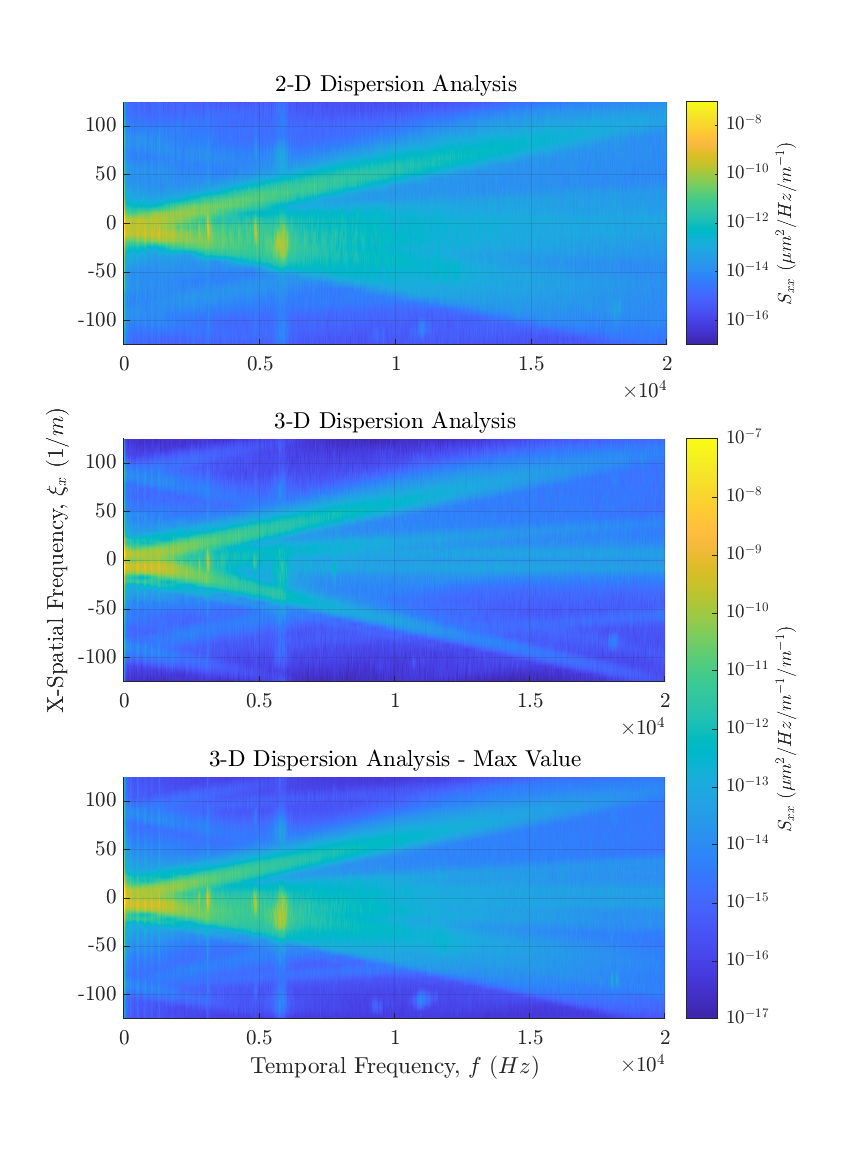
\includegraphics{../matlab/04_dispersion_analysis/dispersion_comparison.eps}
  \caption{Horizontal moving optical disturbances comparison. The top plot shows a slice of the three-dimensional spectrum focusing on the plane waves that are traveling in the horizontal direction. The middle plot is a recreation of the two-dimensional spectrum by integrating through the the vertical spatial-frequencies. The bottom plot is the two-dimensional spectrum.}
  \label{fig:04_dispersion_comparison}
\end{figure}
The top plot shows the three-dimensional spectral estimation plot at $\xi_y=0\ m^{-1}$, which shows planar waves traveling in the horizontal direction.
The middle plot shows the three-dimensional spectrum integrated through the vertical spatial-frequency axis creating an estimate of the two-dimensional spectrum.
The bottom plots shows the two-dimensional spectral plot that was previously shown in Figure \ref{fig:04_dispersion_demo} but this time with a linear temporal-frequency axis.
Both of the two-dimensional spectrum whether directly computed or integrated show a significant increase in the signal content between the acoustic lines ($u\pm c$).

The three-dimensional spectral slice shows signal at the same limits characteristic velocity limits of the free-stream velocity, $u$, and the acoustic lines, $u\pm c$, as the two-dimensional spectrum of signal along with some signal laying along the temporal-frequency axis at $\xi_y=0\ m^{-1}$.
This signal represents a collection of stationary modes at each temporal-frequency.
If this were a flow-related phenomenon the velocity of the disturbance according to Equation \ref{eqn:04_velocity_assumed} would be near infinity; as such, it is more likely caused by mechanical vibration of the wind tunnel and components of the optical measurement system.
On the three-dimensional spectrum plot there are signals that run parallel to $u$ and $u-c$ that do not emanate origin but from $\xi_x\approx\pm80\ m^{-1}$ that show the assumed velocity is not always valid.
\textcolor{red}{I can't think of a good explanation for these other than some mean lensing feature that is both convecting and traveling at $u-c$ and maybe $u+c$. Could be a ghost beam at a different magnification.}
There is also an aliased signal that runs parallel to $u+c$ starting at $\xi_x\approx-50\ m^{-1}$ and decaying towards the left.
Aliased signals are due to the sample rate, either spatial or temporal, being to low.

The middle plot of Figure \ref{fig:04_dispersion_comparison} shows the integrated spectrum through vertical spatial-frequency axis which effectively recreates the two-dimensional spectrum plot.
A reduced order spectrum can be calculated by
\begin{equation}
  S_{xx}^{n-1} = \int S_{xx}^n df_s^m \textrm{,}
\end{equation}
where $S_{xx}^n$ is the n-dimensional spectrum and $df_s^m$ is the differential frequency in the $m$-th dimension.
This can also be shown in Figure \ref{fig:04_dispersion_max}.
\begin{figure}
  \centering
  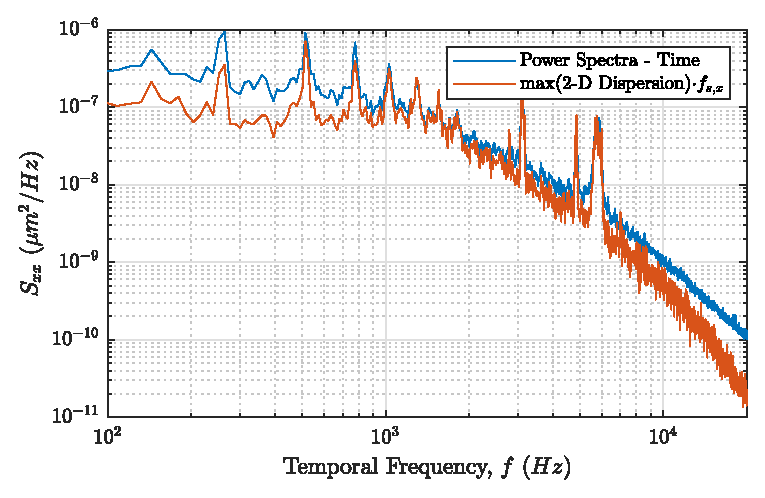
\includegraphics{../matlab/04_dispersion_analysis/dispersion_max.eps}
  \caption{Recovery of time-based power spectrum from two-dimensional spectral estimate.}
  \label{fig:04_dispersion_max}
\end{figure}
While the integrated signal over estimated the spectrum going from three-dimensions to two in Figure \ref{fig:04_dispersion_comparison}, it under estimated the spectrum going from two to one dimensions.
Unfortunately, due to the limited number of spatial sample points and the large dynamic range of the signal, this integrated value can contain a significant of error.

Due to the the signal being relatively sparse, a reduced order spectrum can be estimated by
\begin{equation}
  S_{xx}^{n-1} \approx \max(S_{xx}^n,m)f_s^m \textrm{,}
\end{equation}
where $\max(S_{xx}^n,m)$ is the maximum value of the spectrum along dimension $m$ and $f_s^m$ is the sample rate for that dimension.
The calculated temporal power spectrum from the two-dimensional spectrum using the maximum value is a good estimation at the center of the frequency range but has some additional decay at both low and high frequencies.
The calculated reduced order spectrum appears to follow the functional form of actual spectrum but with a significant offset.

\subsection{2-D Slices of the Multidimensional Spectral Estimation}
The full multidimensional spectrum contains information of flow features that are not only moving in the horizontal direction as the two-dimensional dispersion showed but also in every direction of the two-dimensional optical wavefront.
Figure \ref{fig:04_dispersion_xy} shows two-dimensional slices of the full spectrum that on the top show the horizontal (stream wise) moving disturbances at $\xi_y=0$ $m^{-1}$ and on the bottom show the vertical (cross-stream) moving disturbances at $\xi_x=0$ $m^{-1}$.
\begin{figure}
  \centering
  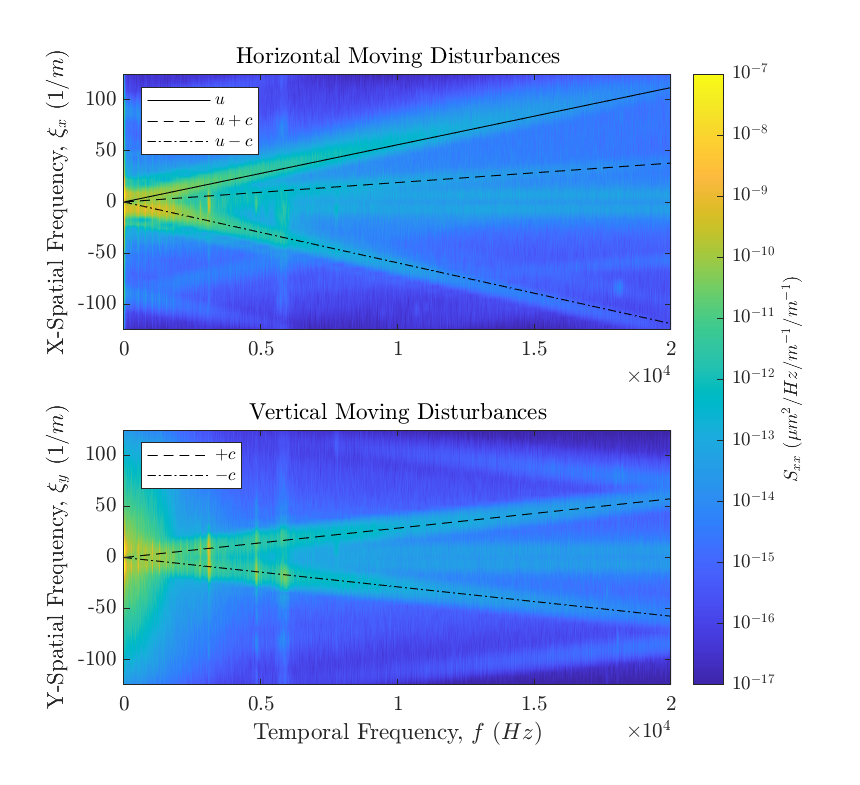
\includegraphics{../matlab/04_dispersion_analysis/dispersion_xy.eps}
  \caption{Horizontal and vertical moving optical disturbances. This is the same data as presented in Figure \ref{fig:04_dispersion_demo} but after calculating the full three-dimensional spectral estimate. These optical disturbances are plane waves that are traveling solely in their respective directions.}
  \label{fig:04_dispersion_xy}
\end{figure}
Since the wavelength is $\lambda=1/\xi$, the waves that make up the disturbances shown in these slices are plane waves that are traveling solely in the these directions.

The top plot shows the two-dimensional spectrum for horizontally moving optical disturbances that was been shown previously.
There are three major flow-related structures that can be observed.
The flow-related structure that lays along $u$ is caused by the boundary layers on both walls of the wind tunnel.
It can be seen that the boundary-layer signal has a peak at the free-stream velocity, $u$, and has a slight decay as the velocity decreases towards the dotted line of $0.7u$ with a sharp decay as the velocity increases.
While the boundary layer velocity has typically be reported as approximately 0.83$u$ \cite{Gordeyev-2014-jcJndkHM}, this data shows the boundary layer velocity has a range of velocities at each given frequency in which the peak velocity component has some dependence on the temporal frequency.
This can be more clearly seen in two temporal-frequency slice in Figure \ref{fig:04_dispersion_slices_velocity}.
\begin{figure}
  \centering
  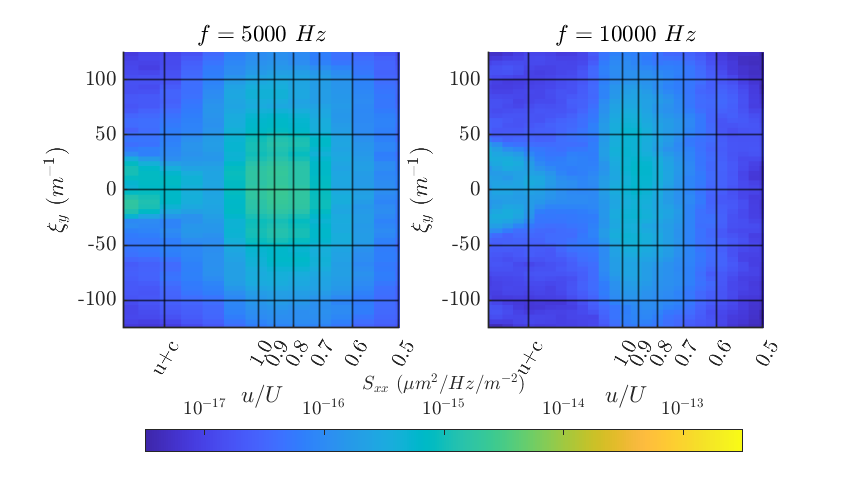
\includegraphics{../matlab/04_dispersion_analysis/dispersion_slices_velocity.eps}
  \caption{Temporal-frequency slices at 5 and 10 kHz with the various horizontal velocities labeled.}
  \label{fig:04_dispersion_slices_velocity}
\end{figure}
Here the horizontal spatial-frequency has been replaced with the normalized horizontal velocity.
The significant decay of the signal as the speed increases above the free-stream velocity there is a gradual decay as the speed decreases.
There is also additional signal decay as the absolute value of the vertical spatial-frequency increases.
The velocity of this boundary layer optical disturbance will be measured in Chapter \ref{chap:06_single_filter} using a velocity filter to show a mean velocity of $0.85u$, which is near the generally accepted value of $0.83u$ \cite{Gordeyev-2014-jcJndkHM}.

The other two major flow-related structures in Figure \ref{fig:04_dispersion_xy} are related to acoustic signals traveling in both directions through the wind-tunnel, denoted by the dashed and dot-dash lines in the figure.
The downstream-traveling acoustic wave, $u+c$, has a low signal power than the upstream-traveling acoustic wave, $u-c$.
The likely explanation for this difference in signal power is that most of the acoustic energy in the wind tunnel is generated by the fan which propagates upstream and downstream within the wind-tunnel ducting.
However, sound waves that move in the flow direction have their wavelength stretched as the flow is accelerated into the test-section contraction, while sound waves moving against the flow have their wavelength contracted.
Hence the downstream-traveling waves have a longer wavelength as they pass through the measurement beam and thus more of the optical signal from the downstream-travelling waves is filtered out due to aperture filtering \cite{Siegenthaler-2008-9Yutbt6c}.
At low temporal-frequencies, the blade-passing frequency (~520 Hz) and its associated harmonics appear as vertical lines with regular spacing in Figure \ref{fig:04_dispersion_xy}.
% There also appears to be some constructive interference with the BPF and some of the aliased data around $\xi_x = \pm100\ m^{-1}$.

The two main features on the vertical spectral slice plot on the bottom of Figure \ref{fig:04_dispersion_xy} are the signals moving at the speed of sound ($\pm c$) including some significant aliasing of these signals.
These two lines represent acoustic waves that are traveling either straight up or down through the measurement beam.
The blade-passing frequency and its harmonics are also visible in the vertical moving wave plots in both directions and have much less broadband spatial content in the vertical direction.
Some of the high temporal-frequency narrow-band signals (~3, 5, and 6 kHz) contain most of the signal power at the speed of sound lines in the vertical spectral slice plot.
These signals has some dependence on the free-stream Mach number (see Figure \ref{fig:04_dispersion_mach}).
These maybe vibrations originating from the tunnel fan that are currently limiting the top speed of the tunnel; some older optical wavefronts collected in this tunnel under similar measurement conditions do not show these narrow-band signals.
Because the portion of these signals with the most power is traveling vertically through the test section instead of steam wise, the tunnel walls maybe excited by the fan and resonating.

The stationary modes that have been discussed previously that lay along the temporal-frequency axis in the horizontal spectral slice plot also appear in the same location in the vertical spectral slice plot.
These stationary modes appear the be constant when viewed from either direction and through out time.
As a white-noise is generally not physical unless it is bandwidth limited with a falloff of at least $1/f^2$ \cite{Blackman-1958-4QtKgDb8}.
Some of these stationary modes are likely cause by vibrations of various optical elements, especially at low temporal-frequencies.
At higher temporal-frequencies, the stationary modes maybe related to electronic noise from the high-speed camera, higher order optical noise from the laser, or even numerical error from the processing code.

\subsection{3-D Representations of Multidimensional Spectral Estimation}
While the two-dimensional slices are fairly informative, particularly when it comes to signal strength of various flow structures and their velocities, a three-dimensional plot allows better visualization of the overall flow structures although some details are lost because typically only one power level can be plotted at a time.
The same data that has been previously shown in two-dimensional form, is depicted in Figure \ref{fig:04_dispersion_3d} as an isosurface with a power of $10^{-14}$ $\mu m^2/Hz/m^{-1}/m^{-1}$ and shown from four different views.
\begin{figure}
  \centering
  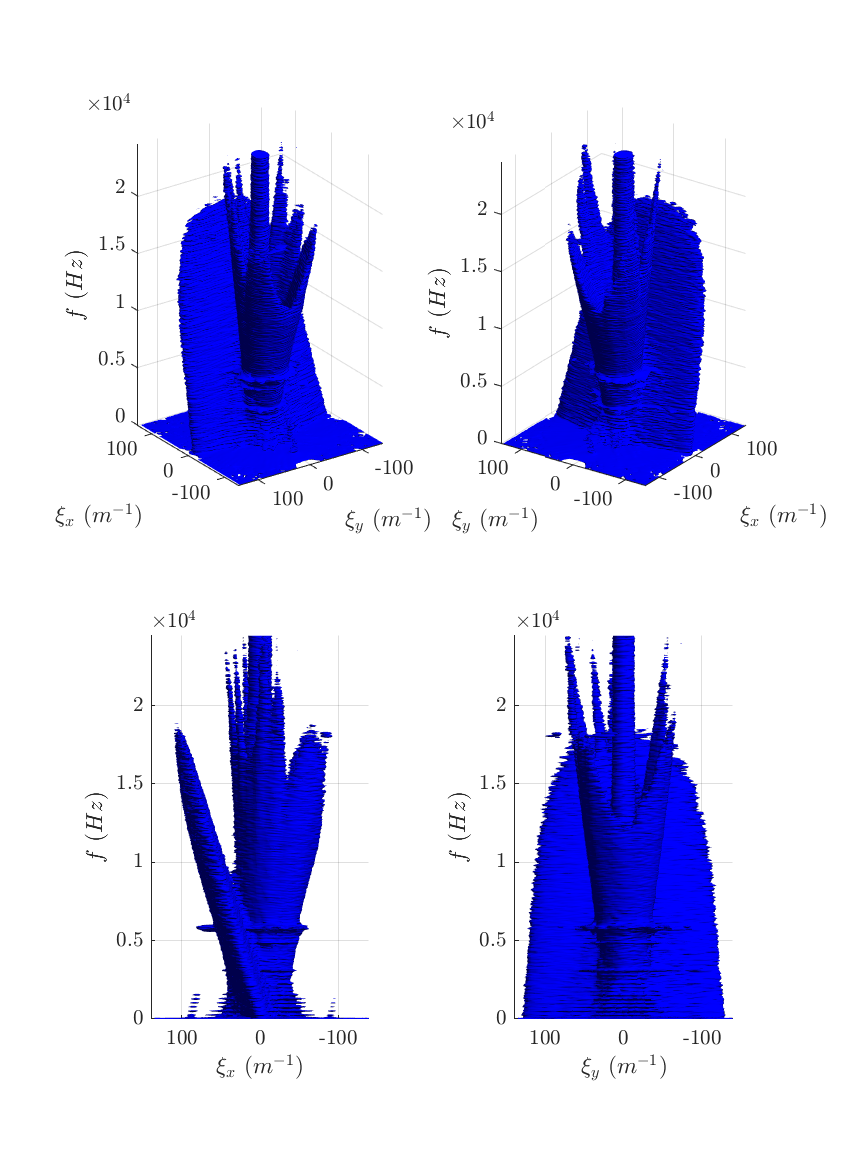
\includegraphics{../matlab/04_dispersion_analysis/dispersion_3d.eps}
  \caption{Three-dimensional view of the multidimensional spectral plot showing an isosurface at a power of $10^{-14}$ $\mu m^2/Hz/m^{-1}/m^{-1}$. The isosurface encompasses 99.9\% of the power of the wavefront.}
  \label{fig:04_dispersion_3d}
\end{figure}
This particular isosurface encompasses approximately 99.9\% of the power of the optical disturbances.
The largest feature is the boundary layer which resembles an ellipsoidal plane that is tilted in the $f-\xi_s$ plane.
The other main feature is the acoustic signal which appears as a cone which is slightly tilted in the direction of upstream-moving disturbances.
The acoustic signal separates into several spikes at high temporal frequencies some of which are constructive interference from aliased signal ($\xi_x\approx25\ m^{-1},\ \xi_y\approx\pm60\ m^{-1}, \textrm{and}\ f\approx20 kHz$) which is better visualized in the 20 kHz temporal-frequency spectral slice in Figure \ref{fig:04_dispersion_slices_velocity}.
There may also be a small number of dominant duct modes at these high temporal-frequencies.
The last feature is the stationary modes which appears as the cylindrical structure along the center of the plot (near zero spatial-frequency in x and y), which have a near constant shape and magnitude through all temporal-frequency ranges.

Figure \ref{fig:04_dispersion_mach} shows two views of an isosurface of the multidimensional spectrum over a range of Mach numbers.
\begin{figure}
  \centering
  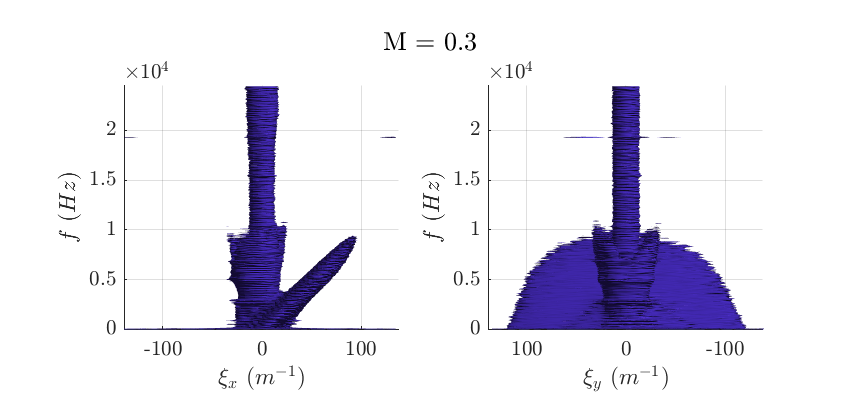
\includegraphics{../matlab/04_dispersion_analysis/dispersion_mach_0.3.eps}
  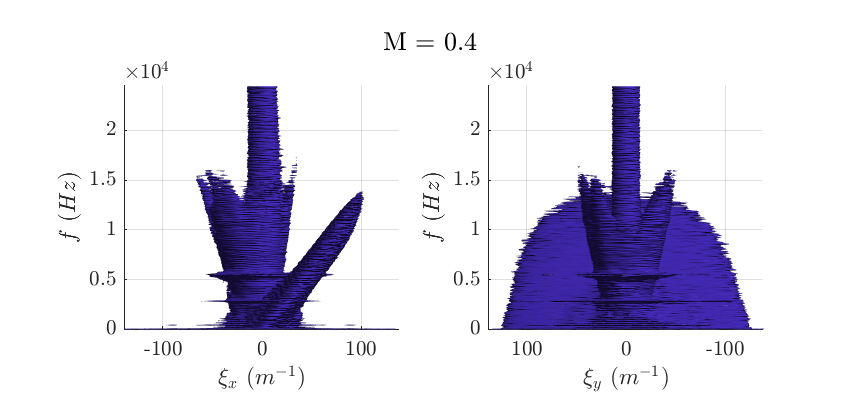
\includegraphics{../matlab/04_dispersion_analysis/dispersion_mach_0.4.eps}
  \includegraphics{../matlab/04_dispersion_analysis/dispersion_mach_0.5.eps}
  \caption{Multidimensional spectral estimate isosurfaces as the Mach number increased from 0.3 to 0.5. The isosurfaces are all shown at a power of $10^{-14}$ $\mu m^2/Hz/m^{-1}/m^{-1}$ and all encompass 99.9\% of the wavefront power.}
  \label{fig:04_dispersion_mach}
\end{figure}
All of these plots are of an isosurface with the same power as used in Figure \ref{fig:04_dispersion_3d}.
The stationary modes seems to be constant throughout the range of Mach numbers indicating that they are most likely not flow related.
The boundary layer signal increases in power significantly as the Mach number is increased while also the slope and thus the velocity is significantly increased as well.
As shown in \cite{Gordeyev-2014-jcJndkHM}, the aero-optical $\opdrms$ of the flat-plate boundary layer on the walls of the wind tunnel is expected to vary according to
\begin{equation}
  \opdrms = BK_{GD}\rho_\infty M^2\delta\sqrt{C_f}G(M) \textrm{.}
  \label{eqn:04_opdrms_bl}
\end{equation}
Hence the significant increase in the power of the boundary-layer spectrum with Mach number that can be observed in Figure \ref{fig:04_dispersion_mach} is expected based on the $M^2$ dependence in Equation \ref{eqn:04_opdrms_bl}.
The increase in slope of the boundary-layer signal is also expected, and is caused by the increase in the convection speed of the boundary-layer aero-optical disturbances as the free-stream Mach number increases.
The acoustic signal sees some interesting evolution as well.
Along with the strength greatly increasing with Mach number, the slope of the upstream traveling disturbances decreases significantly while the downstream moving acoustic disturbances do not see much change other than an increase in signal strength.

As the angle of the optical beam changes as it looks through the test section the horizontal spatial-frequency goes from measuring only the axial component of the optical disturbance to measuring a combination of the axial and span wise component.
This can be seen in Figure \ref{fig:04_dispersion_angle} with the same isosurface value as shown in previous figures and at a Mach number of 0.5.
\begin{figure}
  \centering
  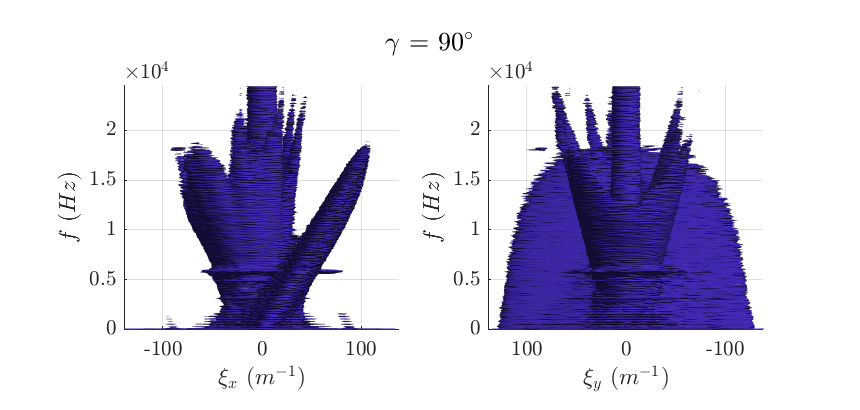
\includegraphics{../matlab/04_dispersion_analysis/dispersion_angle_90.eps}
  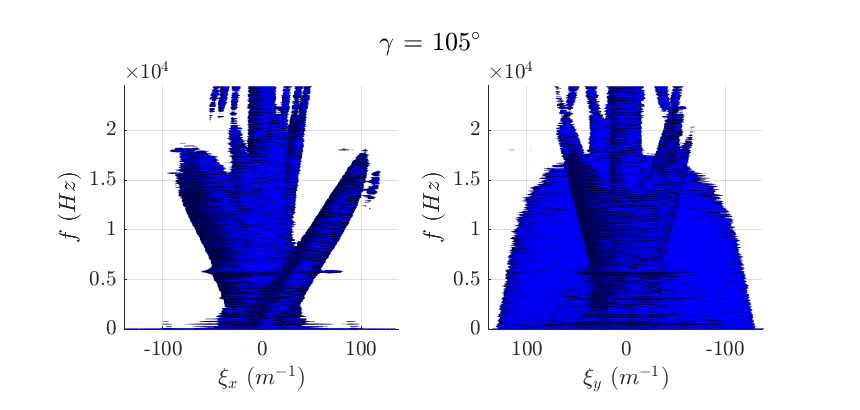
\includegraphics{../matlab/04_dispersion_analysis/dispersion_angle_105.eps}
  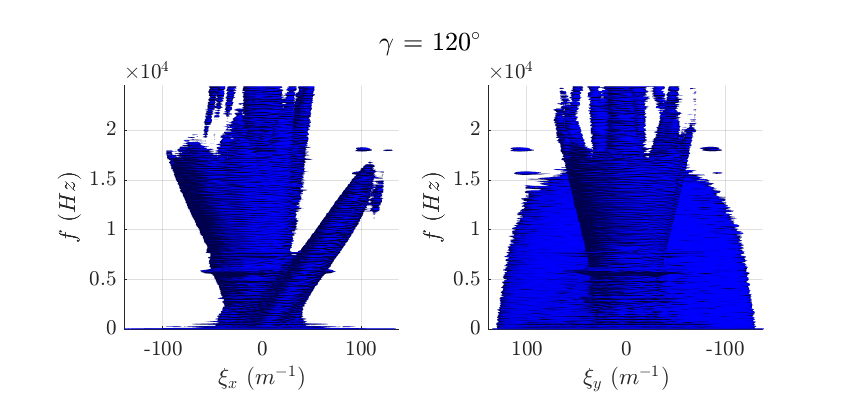
\includegraphics{../matlab/04_dispersion_analysis/dispersion_angle_120.eps}
  \caption{Multidimensional spectral estimate isosurfaces of different viewing angles through the test section at a Mach number of 0.5. The isosurfaces are all shown at a power of $10^{-14}$ $\mu m^2/Hz/m^{-1}/m^{-1}$ and all encompass 99.9\% of the wavefront power.}
  \label{fig:04_dispersion_angle}
\end{figure}
The $90^\circ$ case has been shown previously and the vertical component of the optical  disturbance sees little change as the viewing angle is increase except a small reduction in the boundary layer signal and some additional signal at the high temporal-frequencies in the acoustic cone.
As the angle is increased the side of the acoustic cone traveling in the direction of flow is significantly in power, with a large amount of the signal being aliased into the upstream-traveling side as `stalactites' as odd angles.
The upstream-traveling acoustic signal is also increased in power but to a lesser extent.
The stationary mode pillar experiences some change as well as the viewing angle hits $120^\circ$ and is stretched in the horizontal direction.
The effective velocity of the optical disturbances is reduced for the disturbances traveling in the same direction as the flow and increased for the disturbances traveling in the opposite direction.


While these three-dimensional isosurfaces offer some significant insight into the overall structure of the various optical disturbances they do not show how the spectral inside of the isosurface is distributed.
Views inside of the isosurface of the horizontal and vertical plane waves were shown in Figure \ref{fig:04_dispersion_xy} while Figure \ref{fig:04_dispersion_slices} shows slices at various temporal-frequencies.
\begin{figure}
  \centering
  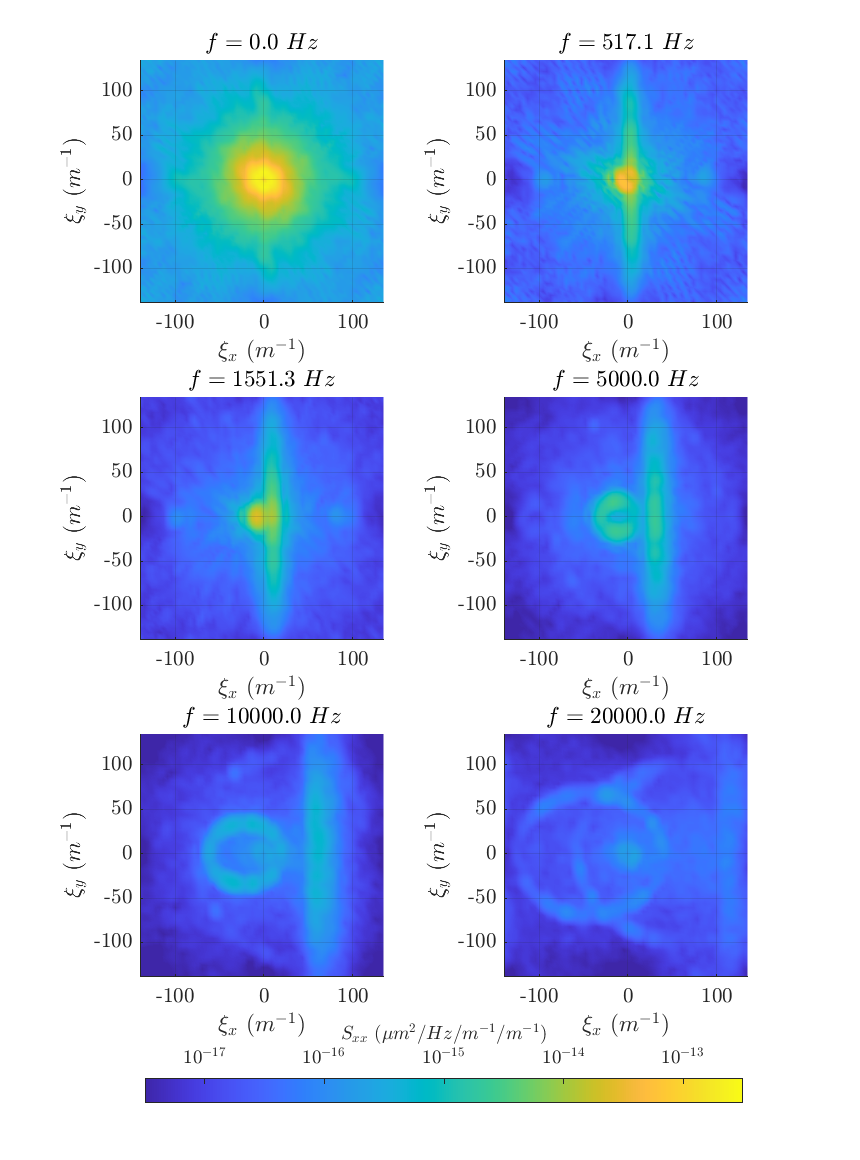
\includegraphics{../matlab/04_dispersion_analysis/dispersion_slices.eps}
  \caption{Multidimensional spectral estimate slices at various temporal-frequencies.}
  \label{fig:04_dispersion_slices}
\end{figure}
The temporal-frequencies spectral slices shown are at: 0 Hz, the blade-passing frequency at 517 Hz, the second harmonic of the blade-passing frequency at 1551 Hz, and additional slices at 5, 10, and 20 kHz.
The slice at 0 Hz temporal frequency shows the spatial frequencies of the wavefront disturbance that does not change with time.
This temporally constant wavefront disturbance is typically called the ``mean lensing''component of the wavefront measurement, since it is has an effect similar to a lens placed in the beam.
The mean lensing slice at 0 Hz shows a mostly axisymmetric pattern with most of its power concentrated at low spatial frequencies.
There appear to be the occasional spike radiating out from the center, most noticeably in line with the boundary layer signal.

The next four slices, for $f$=517.1 Hz to 10 kHz, show a vertical line associated with the boundary layers aero-optical disturbance, which  progressively moves towards positive x-spatial frequencies with increasing frequency.
The boundary-layer disturbance appears to be rotated slightly counter-clockwise indicating that the interrogation beam is slightly rotated between the test section and the wavefront sensor.
The boundary layer signals at the lower temporal-frequencies appear to have equal decay in both the positive and negative $\xi_x$ directions while at the higher frequencies, the decay is much more gradual in the positive $\xi_x$ direction.
This could be indicative of the lower temporal-frequency disturbances in the boundary layer typically traveling at a more uniform speed very near the free-stream velocity likely being either in the outer boundary layer or free-stream tunnel turbulence.
The higher temporal-frequency disturbances seem to have a much wider range of velocities that approach the free-stream velocity and are likely small structures that reside in different parts of the boundary layer and hence travel with a wide range of convection velocities.

The acoustic disturbances show an interesting evolution as the temporal-frequency increases.
At low temporal-frequencies, the acoustic disturbances are concentrated near zero spatial frequency and with strong power.
At high temporal-frequencies the acoustic disturbances appear as elliptically shaped rings.
At 20 kHz, there are two elliptical shapes that are easily identifiable, the smaller one is the signal that is actually present at that frequency while the other one is aliased data due to the limited temporal sample rate.
There is constructive interference where the two acoustic ring intersect.
The 10 kHz slice also shows a small amount of acoustic aliasing
Both the 10 and 20 kHz acoustic rings show some a non-uniform signal power throughout the circumference which are also visible in the three-dimensional views as the spikes at the high temporal-frequencies.
% Both of these temporal spectral slices show the center stationary mode column that appears to be nearly identical.

\subsection{Acoustic Cone}
The shape of the acoustic cone can be visualized by plotting the relationship between the temporal frequency and the vertical and axial wavenumbers for a beam going through a duct at $90^\circ$.
Figure \ref{fig:04_dispersion_sound} shows the acoustic cone mode lines for a small set of duct modes at various Mach numbers for a duct that is 1 meter square.
\begin{figure}
  \centering
  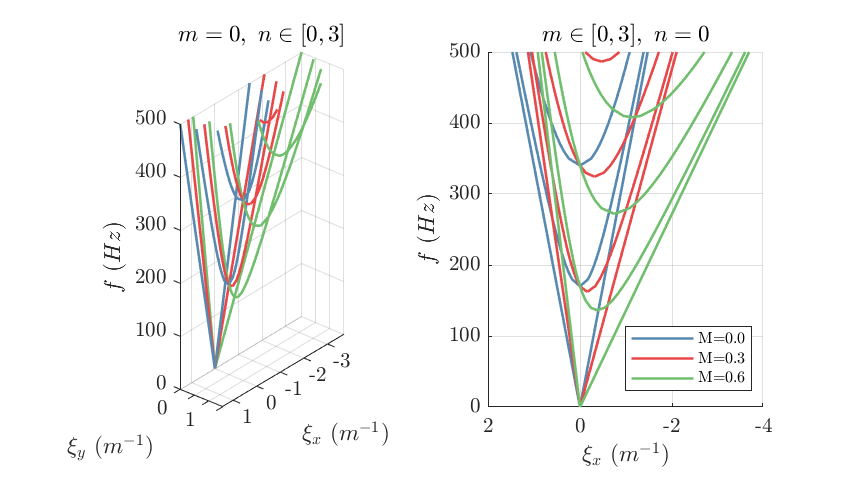
\includegraphics{../matlab/04_dispersion_analysis/dispersion_sound.eps}
  \caption{Acoustic duct mode lines showing the spatial-frequency location as a function of temporal-frequency, Mach number, and mode number.}
  \label{fig:04_dispersion_sound}
\end{figure}
The cross-sectional wavenumbers are $k_x = m\pi/l_x$ and $k_y = n\pi/l_y$ with the vertical spacial-frequency , $\xi_y=k_y/2\pi$.
The horizontal spacial-frequency is related to the axial wavenumbers, Equation \ref{eqn:02_kzm}, for sound traveling upstream or downstream.

The plot on the left of Figure \ref{fig:04_dispersion_sound} shows the acoustic cone when $m=0$ and $n\in [0,3]$ at Mach numbers of 0, 0.3, and 0.6.
Only shown is the positive vertical spatial-frequency.
As the vertical spatial-frequency of a duct-mode varies only with the mode number $n$ each set occupies a distinct plane, $\xi_y=n/2l_y$.
Only acoustic cone modal lines representing the cut-on duct modes are shown.

The plot on the right of Figure \ref{fig:04_dispersion_sound} shows the acoustic modal lines at $\xi_y=0$ for $n=0$ which fill the inside of the acoustic cone.
The Mach number has a far greater impact on the acoustic cone for the waves traveling upstream.
As the Mach number increases, the cut-on frequency (minimum value in $f$) decreases and the horizontal spatial-frequency at the cut-on frequency also decreases.
This effect is more pronounced at higher mode numbers.
The phase velocity of a downstream-traveling acoustic wave can travel upstream.

It maybe possible to individually resolve the separate acoustic duct modes using optical wavefronts if the spatial frequency resolution where high enough.
To measure of the vertical mode number, $n$, the spatial-frequency resolution would need to be $\Delta\xi_y\ge 1/2l_y$ for a square duct.
With a single beam going through the duct perpendicularly, the axial wave number is directly measurable but its sensitivity is diminished as the temporal-frequency is increased.
It would be most sensitive to measuring modes that have just been cut-on.

\subsection{Signal Aliasing}
In the spectral slices shown in Figure \ref{fig:04_dispersion_xy}, when a signal crosses a plane represented by one of the Nyquist frequencies (positive or negative) it is transposed to the conjugate Nyquist frequency plane and continues on with the same gradient as before.
This behavior is illustrated in Figure \ref{fig:04_dispersion_supersample} using tiled horizontal and vertical multidimensional spectrum slices.
\begin{figure}
  \centering
  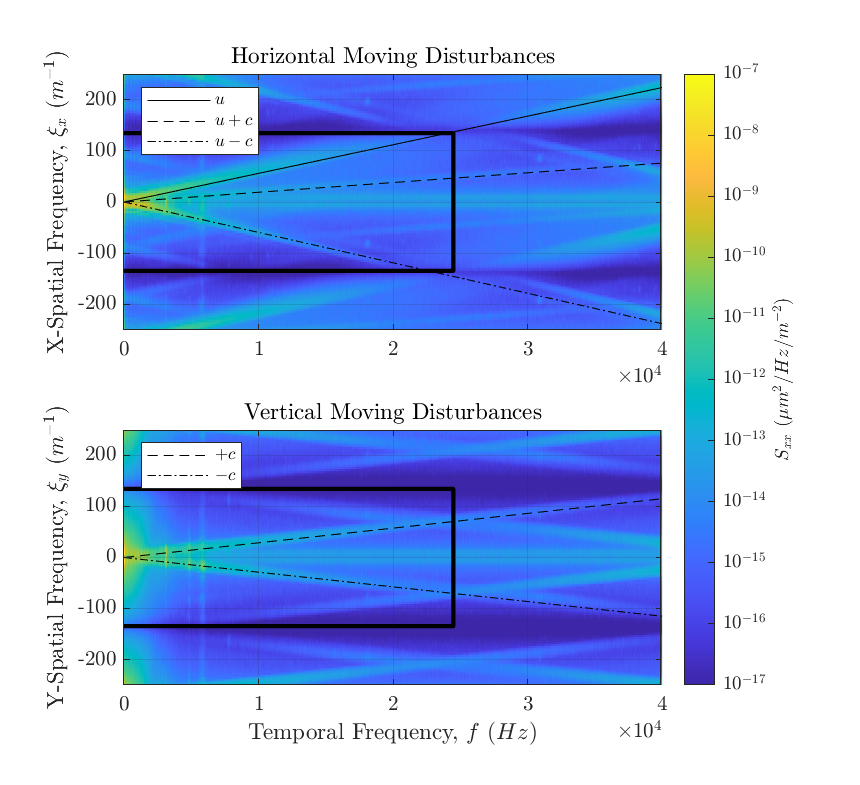
\includegraphics{../matlab/04_dispersion_analysis/dispersion_supersample.eps}
  \caption{Artificially increased temporal sample rate using a dispersion analysis. The black box represents original dispersion plot.}
  \label{fig:04_dispersion_supersample}
\end{figure}
The tiling process for the spectral slices,
\begin{equation}
  S_{xx}^{\xi_y=0} = \left[
    \begin{array}{c c c}
      S_{xx}^{\xi_y=0} & S_{xx}^{\xi_y=0} & S_{xx}^{\xi_y=0} \\
      S_{xx}^{\xi_y=0} & S_{xx}^{\xi_y=0} & S_{xx}^{\xi_y=0} \\
      S_{xx}^{\xi_y=0} & S_{xx}^{\xi_y=0} & S_{xx}^{\xi_y=0}
    \end{array}
  \right] \textrm{,}
\end{equation}
where $S_{xx}^{\xi_y=0}$ is the spectral slice showing the horizontal moving disturbances at $\xi_y=0$.
The temporal frequency is tiled,
\begin{equation}
  f = \left[
    \begin{array}{c c c}
      f-f_s & f & f+f_s
    \end{array}
  \right] \textrm{,}
\end{equation}
where the other frequencies are similarly tiled.
This tiling process could be used on the full multidimensional spectrum with the tiling occurring on each axis.
This process has the effect of artificially increasing the sampling rate while also duplicating all of the data many times \cite{Lynch-2021-DygYkEGU}.

In Figure \ref{fig:04_dispersion_supersample}, the black box represents the original extents of the spectrum along with lines representing the free-stream velocity and the sonic lines.
When these characteristic lines are extended past the original sample rate, aliased information becomes more apparent.
On the upstream moving disturbance side there is some noticeable aliasing that is present including a significant spike at 18 kHz (-80 $m^{-1}$) while aliased and about 31 kHz (-200 $m^{-1}$) when it has been unaliased.
As that upstream moving acoustic disturbance crosses the spatial Nyquist frequency, the signal strength drops significantly to local background levels.
The boundary layer signal is unfortunately to well aligned with its tiled self for any aliased data to be noticeable.
The vertically moving disturbances have some significant temporal aliasing but little to no spatial aliasing.

There maybe some circumstances when aliased data cannot even be identified, such is likely the case for the boundary layer signal shown in the horizontal moving disturbances plot because the signal is directly inline with its aliased self.
This may also cause an issue when trying to analyze the original spectrum, particularly at the higher frequencies where the aliased data is sufficiently strong and overlapping the true signal.
To avoid this the sample rate velocity,
\begin{equation}
  V_s=f/\xi \textrm{,}
\end{equation}
should sufficiently different enough from the disturbance's characteristic velocity.
This difference will vary for the depending on the spectral width of the signal.
The sample rate velocity of the spectrum in Figure \ref{fig:04_dispersion_supersample} is 176.4 m/s, the free-stream velocity is 174.3 m/s and the boundary layer has a significant spectral with to the signal such that it would be difficult to separate the real and aliased signals.
The upstream-traveling acoustic wave however is a fairly thin signal that is distinguishable from the aliased signal and it has a characteristic velocity of -173.0 m/s.

\section{Summary}
The use of multidimensional spectral estimation on optical wavefronts can provide significant additional insight to the various components that are being measured, including the desired aero-optical signal but also various forms of noise including sound and vibration.
The process of filtering these multidimensional spectra will be discussed in Chapters \ref{chap:06_single_filter} and \ref{chap:07_multiple_filter}. 
